\chapter{Standard Model \& Vector Boson Scattering} % (fold)
\label{cha:standard_model__vector_boson_scattering}
\begin{chapquote}
{C.N. Yang}
Now if we adopt the view that this arbitrary convention should be independently chosen at every space-time point, then we are naturally led to the concept of gauge fields.
\end{chapquote}
In this chapter, a brief introduction of the SM with the EWSB is given. Also, the aQGC and VBS is discussed briefly.
\section{Brief Introduction of SM} % (fold)
\label{sec:brief_introduction_of_sm}
SM is the theory of elementary particles and their interactions. It is well tested and in good agreement with experimental results.

Till now we know four fundamental interactions.
Out of four, the gravitational interaction is not included in SM.
The other three forces the strong force interaction is described by Quantum Chromodynamics (QCD), the electromagnetic interaction is described by Quantum Electrodynamics (QED) and the weak interaction are included in the SM.
In 1979 Sheldon Glashow, Abdus Salam, and Steven Weinberg awarded Nobel prize for their effort to unify the theory of weak interaction and the quantum electrodynamics~\cite{StandardModel67_1,StandardModel67_2}.
This unified theory of weak interaction and quantum electrodynamics is known as the electroweak theory.

According to SM all the fundamental particles can be classified into two categories. They are fermions and bosons.

Fermions are the particles that obey the Fermi-Dirac statistics with half-integer spin.
In SM fermions are further classified into leptons and quarks, which are listed in Table~\ref{table:smfermions}.
The quarks and leptons create the subatomic scaffolding for solid matter.
Quarks bind together to form protons and neutrons and the electrons orbit these cluster of quarks to form atoms and the atoms combine into all the known stable matter of universe~\cite{SM-buildingblock_uslhc}.
Till now we know the three generations of leptons as well as quarks. The different generations are differing only in the particle mass.
\begin{table}
% \vspace{-5.2em}
\centering
\begin{tabular}[!htbp]{l l l l l l}
\hline
{\textbf{Generation}} & {\textbf{Fermion}} & {\textbf{Electric}} & \multicolumn{2}{c}{\textbf{Weak isospin $|I_3|$}} & \textbf{Mass in MeV} \\
    &           &    \textbf{Charge}  & \textbf{left-} & \textbf{right-} &     \\
    &           &                     & \textbf{handed} & \textbf{handed} &    \\
\hline
\multirow{4}{*}{$1^{st}$} & electron ($e^-$)           &   -1 & 1/2 &  0    &   $0.511\pm 3.1\times 10^{-8}$ \\
         & electron-neutrino ($\nu_e$)&   0  & 1/2 &  none &   $<2 \times 10^{-6}$   \\
         & up quark ($u$)             &  2/3 & 1/2 &  0    &   $2.2^{+0.5}_{-0.4}$  \\
         & down quark ($d$)           & -1/3 & 1/2 &  0    &   $4.7^{+0.5}_{-0.3}$  \\
\hline
\multirow{4}{*}{$2^{nd}$} & muon ($\mu^-$)             &  -1  & 1/2 &  0    &   $105.658 \pm 2.4 \times 10^{-6}$ \\
         & muon-neutrino ($\nu_{\mu}$)& 0    & 1/2 &  none &   $<2 \times 10^{-6}$   \\
         & charm quark ($c$)                & 2/3  & 1/2 &  0    &   $1275^{+25}_{-35}$     \\
         & strange quark ($s$)              & -1/3 & 1/2 &  0    &   $95^{+9}_{-3}$       \\
\hline
\multirow{4}{*}{$3^{rd}$} & tau ($\tau^-$)             & -1   & 1/2 &  0    &    1776.86 $\pm$ 0.12    \\
         & tau-neutrino ($\tau_{\mu}$)& 0    & 1/2 &  none &   $<2 \times 10^{-6}$   \\
         & top quark ($t$)                  & 2/3  & 1/2 &  0    &   $1.73\times 10^5\pm 40$\\
         & bottom quark ($b$)               & -1/3 & 1/2 &  0    &   ${4.18 \times 10^{3}}^{+40}_{-30}$\\
\hline
\end{tabular}
\caption{Fermions list in SM~\cite{PDG2018}.}
\label{table:smfermions}
\end{table}

Bosons are the particles that obey the Bose-Einstein statistics with integer spin. In SM the bosons are the mediator of interactions between the particles, described by a local gauge theory. Thus, these bosons are called gauge bosons. All the bosons in SM are listed in Table~\ref{table:smbosons}.
The photon and gluons are massless carrying electromagnetic and strong force respectively. The $W^{\pm}$ and $Z$ bosons carry the weak force. These bosons are the spin 1 bosons and known as the vector-bosons. Whereas, the Higgs boson, H, is a scalar boson with spin 0. This is responsible for the mass generation (by giving longitudinal polarization) to the fundamental particles through EWSB, which is explained in section~\ref{sub:brief_introduction_to_higgs_mechanism}.

\begin{table}
% \vspace{-5.2em}
\centering
\begin{tabular}[!htbp]{l l l l l l}
\hline
    & \textbf{Bosons} & \textbf{Electric Charge} & \textbf{Spin} & \textbf{Interaction} & \textbf{Mass in GeV} \\
\hline
$\gamma$  & photon   & 0      & 1 & electromagnetic   &   $<1 \times 10^{-27}$ \\
$W^{\pm}$ & W bosons & $\pm$1 & 1 & weak              &  80.379 $\pm$ 0.012    \\
$Z^0$     & Z boson  & 0      & 1 & weak              &  91.188 $\pm$ 0.0023    \\
$g$       & gluons   & 0      & 1 & strong            &  0                     \\
\hline
$H$       & Higgs    & 0      & 0 &                    & 125.18 $\pm$ 0.16     \\
\hline
\end{tabular}
\caption{Bosons list in SM~\cite{PDG2018}.}
\label{table:smbosons}
\end{table}

\subsection{Standard Model as Gauge theory}
Gauge invariance is the key ingredient in the construction of the SM of electromagnetic, weak and strong interactions of elementary particles. In general gauge principle specify that for a given gauge symmetry group and the transformation of the fields, the quantum field theory can be uniquely defined~\cite{Coughlan2006}.
% Below the theory of Quantum Electrodynamics (QED) is briefly discussed.

% \subsubsection{Example: Quantum Electrodynamics} % (fold)
% \label{ssub:example_quantum_electrodynamics}
The construction of QED is one of an example of local gauge theory as the Lagrangian function (Eq.~\ref{eq:qed_lagrangian}) that describes the QED of the spin-half particle remains invariant by the local gauge transformation of the electron field $\psi(x)$ and the photon field $A_{\mu(x)}$ at all space-time point x.
\begin{equation}\label{eq:qed_lagrangian}
    \Lagr = i \bar{\psi}\gamma^{\mu} D_{\mu}\psi - m\bar{\psi}\psi,
    % \Lagr = i \bar{\psi}\gamma^{\mu} \partial_{\mu}\psi - m\bar{\psi}\psi
\end{equation}
The transformation followed by the electron field and photon field is:
\begin{eqnarray}\label{eq:qed_phase}
    \psi(x) & \rightarrow & e^{iq\chi(x)}\psi(x), \nonumber \\
    A_\mu(x) & \rightarrow & A_\mu(x) - {\partial_\mu \chi(x)}, 
\end{eqnarray}
Where the $\chi(x)$ is the arbitrary phase transformation, q is the electron-photon coupling.
And the $D_{\mu}$ given in the eq.~\ref{eq:qed_lagrangian} is known as covariant derivative and is given as:
\begin{equation}
    D_{\mu} = \partial_{\mu} + iqA_{\mu},
\end{equation}
Here, the photon field plays an intrinsic role and without which there could be no local gauge invariance. While the construction of the local gauge invariance of QED, we realize that the local gauge invariance of a spin-half particle requires the existence of a gauge boson and there coupling with the fermions. Also, for the exact gauge invariance, the gauge bosons must be massless. 

In Eq.~\ref{eq:qed_phase}, the phase factor $e^{i\chi(x)}$ belongs to the symmetry group $U(1)$ of the unitarity transformations in one dimension. Thus, the generalization of the QED can be made to the other forces by exploring the other possibility of the symmetry group.

For example, the electrons and neutrino can be chosen as a double $(\nu_e,e)$, i.e. as two members of the same family, since both of them are spin-half particles.
Thus, it can be described as the doublet by a two-component field $\phi = (\nu_e(x),e(x))$ and impose a gauge transformation where $\alpha$ is a $2\times 2$ hermitian matrix operating on the $\phi$.

% \subsubsection{Example: Weak Interactions} % (fold)
% \label{ssub:example_weak_interactions}
The weak interaction, SU(2), local gauge transformation can be written for the electron doublet field as
\begin{eqnarray}
    \phi (x) &  = & e^{ig_w \balpha .\boldsymbol{T}} \phi(x) \nonumber \\
             &  \simeq & (I + ig_w \balpha \boldsymbol{.T})\phi(x),
\end{eqnarray}
where $\balpha$ is the arbitrary infinitesimal vector in the isospin space and the $\bt = \{T_1,T_2,T_3\}$ is the three generators of the SU(2) symmetry group, which can be expressed using Pauli spin matrices as $\bt = \bsigma / 2$. Also, the $\bt_i$ do not commute,\begin{equation}
    [T_i,T_j] = i\epsilon_{ijk}T_k,
\end{equation} and the doublet field $\phi(x)$ is given as:
\begin{equation}
    \phi(x) = \begin{bmatrix}
        \nu_e(x)  \\
        e(x)  \\
        \end{bmatrix}.
\end{equation}
As the generator of this group, $T_i$'s do not commute it is said to be the non-Abelian group.

Assuming the fermion mass to be zero the Lagrangian for the electron and electron-neutrino can be written as
\begin{equation}\label{eq:SU2_lag}
    \Lagr = i\bar{\phi}\gamma_{\mu}\partial^{\mu}\phi = i\bar{\nu_e}\gamma_{\mu}\partial^{\mu}\nu_e + i\bar{e}\gamma_{\mu}\partial^{\mu}e
\end{equation}

The $\psi$-field in the Lagrangian, Eq.~\ref{eq:SU2_lag} can be made gauge invariant by using the covariant derivative instead of derivative, which is defined using the three gauge fields given by $\bw = \{W_1,W_2,W_3\}$ as
\begin{equation}\label{eq:su2_covarientderivative}
    \partial_{\mu} \rightarrow D_{\mu} = \partial_{\mu} + i g_w \bw_{\mu}.\bt
\end{equation}

Also the gauge fields $\bw_{i\mu}$ transforms as
\begin{equation}\label{eq:su2_gaugefield}
    \bw_{\mu}(x) \rightarrow \bw_{\mu}(x) + \partial_{\mu}\balpha + g\balpha \times \bw_{\mu}(x)
\end{equation}

Unlike the QED (Eq.~\ref{eq:qed_phase}), the gauge field transformation in weak interaction (or SU(3) group) is complicated because of the non-Abelian property of its generator. Using Eq.~\ref{eq:SU2_lag},\ref{eq:su2_gaugefield}, and~\ref{eq:su2_covarientderivative}, we can show that the Lagrangian of weak interaction, Eq.~\ref{eq:SU2_lag}, remains gauge invariant.

Still, we need to add the kinetic term for the $W$ fields. This can be taken similar to the QED and given by
\begin{equation}\label{eq:su2_kinetic}
    \Lagr_{\bw} = -\frac{1}{4}\bw_{\mu \nu}. \bw^{\mu \nu}
\end{equation}
where,
\begin{equation}\label{eq:su2_kefield_exp}
    \bw_{\mu \nu} = \partial_{\mu} \bw_{\nu} - \partial_{\nu} \bw_{\mu} - g \bw_{\mu} \times \bw_{\nu}
\end{equation}
Here, the term $\bw_{\mu} \times \bw_{\nu}$ shows that the Lagrangian of weak interaction contains the W-boson self-interaction terms and written as
\begin{equation}
    \bw^{\mu} \times \bw^{\nu} = \epsilon_{ijk} W^{\mu}_j W^{\nu}_k
\end{equation}
Now, using Eq.~\ref{eq:su2_kefield_exp}, Eq.~\ref{eq:su2_kinetic} becomes
\begin{eqnarray}
    \Lagr & = & -\frac{1}{4} \Big[ \big( \partial_{\mu} \bw_{\nu} - \partial_{\nu} \bw_{\mu} \big) - g_w \bw_{\mu} \times \bw_{\nu} \Big]  \Big[ \big( \partial^{\mu} \bw^{\nu} - \partial^{\nu} \bw^{\mu} \big) - g_w \bw^{\mu} \times \bw^{\nu} \Big] \nonumber \\
        & = & -\frac{1}{4} \big( \partial_{\mu} \bw_{\nu} - \partial_{\nu} \bw_{\mu} \big) \big( \partial^{\mu} \bw^{\nu} - \partial^{\nu} \bw^{\mu} \big) \nonumber \\
        &   & + \frac{1}{4} \Big[  g_w\big( \partial_{\mu} \bw_{\nu} - \partial_{\nu} \bw_{\mu} \big)\bw^{\mu} \times \bw^{\nu} \Big] + \frac{1}{4} \Big[  g_w \bw_{\mu} \times \bw_{\nu}  \big( \partial^{\mu} \bw^{\nu} - \partial^{\nu} \bw^{\mu} \big)\Big] \nonumber \\
        &   & - \frac{1}{4} g_W^2 \big(\bw_{\mu} \times \bw_{\nu}\big) \big(\bw^{\mu} \times \bw^{\nu}\big) 
\end{eqnarray}
Now, we can explicitly divide the weak interaction Lagrangian into the kinetic and interaction parts, as
\begin{equation}
    \Lagr_W = \Lagr_{kin} + \Lagr_{int},
\end{equation}
where,
\begin{equation}
    \Lagr_{kin} = -\frac{1}{4} \big( \partial_{\mu} \bw_{\nu} - \partial_{\nu} \bw_{\mu} \big) \big( \partial^{\mu} \bw^{\nu} - \partial^{\nu} \bw^{\mu} \big) \nonumber
\end{equation}
and,
\begin{eqnarray}
    \Lagr_{int} & = &  \frac{1}{4} \Big[  g_w\big( \partial_{\mu} \bw_{\nu} - \partial_{\nu} \bw_{\mu} \big)\bw^{\mu} \times \bw^{\nu} \Big] + \frac{1}{4} \Big[  g_w \bw_{\mu} \times \bw_{\nu}  \big( \partial^{\mu} \bw^{\nu} - \partial^{\nu} \bw^{\mu} \big)\Big] \nonumber \\
        &   & - \frac{1}{4} g_W^2 \big(\bw_{\mu} \times \bw_{\nu}\big) \big(\bw^{\mu} \times \bw^{\nu}\big) 
\end{eqnarray}
In component form it can be written as:
\begin{eqnarray}
    \Lagr_{int} & = & \frac{1}{2} \Big[  g_w \epsilon_{ijk}\big( \partial_{\mu} W_{\nu i} - \partial_{\nu} W_{\mu i} \big)W^{\mu}_j \times W^{\nu}_k \Big] \nonumber \\
        &   & - \frac{1}{4} g_W^2 \epsilon_{ijk} \epsilon_{imn} W^{\mu}_j W^{\nu}_k W_{m \mu} W_{n \nu}
\end{eqnarray}
Here, the interaction part of Lagrangian shows that in weak interaction there are triple as well as quartic both types of self-couplings are allowed, as shown in Fig.~\ref{fig:sm_triple_quartic}. In weak interaction, these self-couplings are the consequence of the non-Abelian nature of the SU(2) group algebra. In terms of the physical fields, there are two type of triple gauge couplings, $\gamma \ww$ and $Z \ww$ and three type of quartic gauge couplings, $\ww \ww$, $\ww ZZ$, and $\ww \gamma \gamma$ are allowed in the SM.
\begin{figure}[htbp]
    \centering
    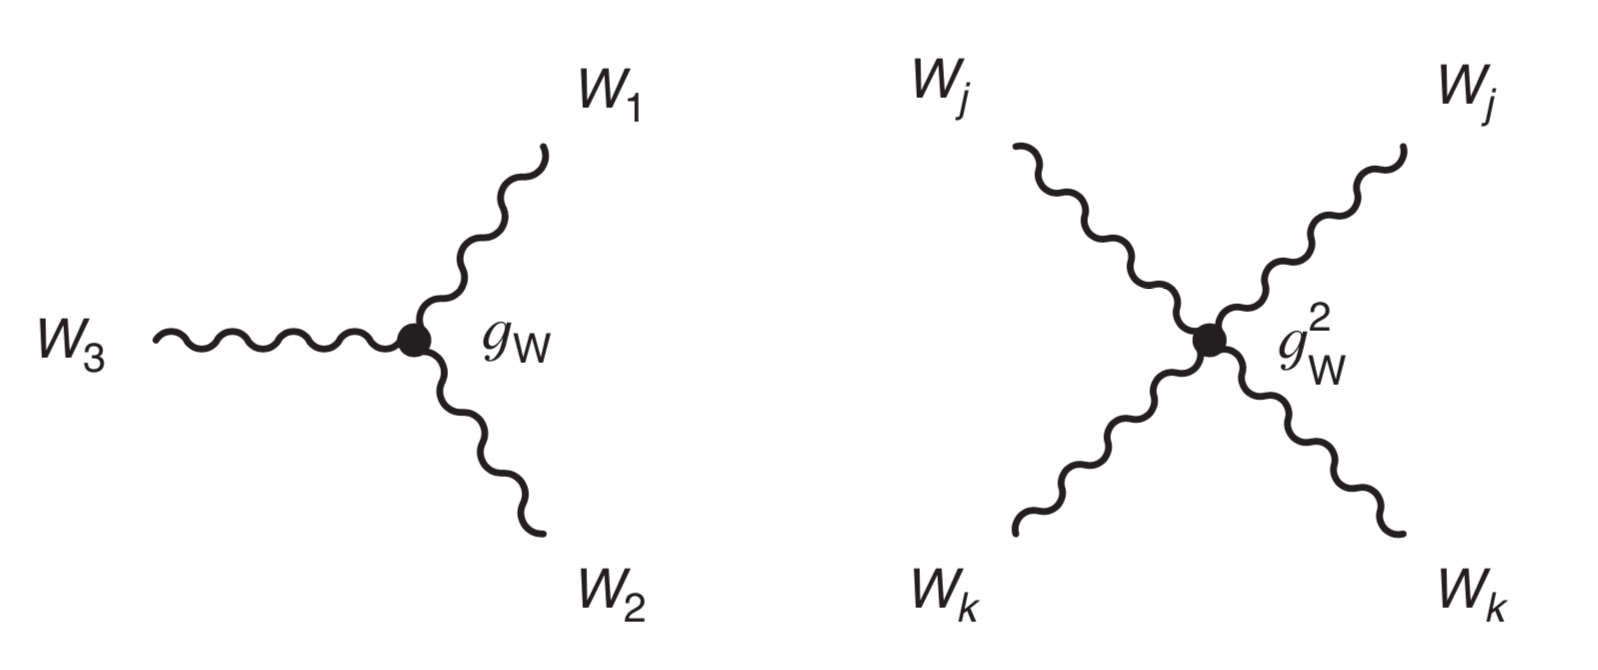
\includegraphics[width=0.95\textwidth]{Pictures/sm-triple-quarticgc.png}
    \caption{sm triple and quartic gauge coupling.}
    \label{fig:sm_triple_quartic}
\end{figure}
% \Big[ \big( \partial_{\mu} \bw_{\nu} - \partial_{\nu} \bw_{\mu} \big) - g \bw_{\mu} \times \bw_{\nu} \Big] \Big[    \big(\partial_{\mu} \bw_{\nu} - \partial_{\nu} \bw_{\mu}\big) - g \bw_{\mu} \times \bw_{\nu} \Big] \nonumber \\


% subsubsection example_weak_interactions_ (end)



%%%%%%%%%%%%%%%%%%%%%%%%%%%%%%%%%%%%%%%%%
%%%%%%%%%%%%%%%%%%%%%%%%%%%%%%%%%%%%%%%%%
%%%%%%%%%%%%%%%%%%%%%%%%%%%%%%%%%%%%%%%%%
Similarly, the other leptons and the quarks can also be put in doublets $(\nu_\mu, \mu),~(\nu_\tau,\tau),~(u,d)$, etc. and subject to the similar transformations.
Furthermore, these transformations are not only the phase factors, as the off-diagonal elements of $\chi$ can change one member of a doublet into the another as it belongs to the same symmetry group SU(2) of the unitary unimodular transformations in 2-dimensions.
And the local gauge invariance in these case requires the introduction of three massless spin-1 gauge bosons $W^+,W^-$ and $W^0$.
Furthermore, if it can be combined with a simultaneous U(1) symmetry and it brings one more gauge boson $B^0$. This group is known as the $SU(2)_L\times U(1)$ gauge group, which is formulated successfully by Glashow, Salam, and Weinberg for the unification of QED and weak interaction (known as electroweak interactions)~\cite{StandardModel67_2} having massless gauge bosons. But all the gauge bosons cannot be massless. As in experiments we measured the masses of gauge bosons $W^+$, $W^-$ and $Z$ bosons. Thus the symmetry cannot be exact. It should be broken spontaneously in such a way that it retains the renormalizable in such a way that it retain three massive bosons $W^+, W^-$ and $Z$ and one massless boson $\gamma$. This is explained in Sec.~\ref{sub:brief_introduction_to_higgs_mechanism}.

The subscript in the $SU(2)_L$ in the electroweak theory tells that the gauge transformation $SU(2)$ only acts on the left-handed particles. This condition is imposed as the process like the beta-decay are observed to involve the quark and leptons with left-handed spins relative to their motions. The first generation of the spin-half particles can be classified in doublet and singlets representations of $SU(2)_L$ as below:
\begin{eqnarray}
    (u_L,d_L),(\nu_{eL},e_L),\bar{u}_L,\bar{d}_L,\bar{e}_L, \nonumber \\
    (\bar{d}_R,\bar{u}_R),(\bar{e}_R,\bar{\nu}_{eR}),u_R,d_R,e_R.   \nonumber
\end{eqnarray}

Furthermore, we did not find the right-handed neutrino state experimentally yet.
Thus we have 15 left-handed (and 15 right-handed) fermion states in each generation counting three colours for each quark flavour, in this gauge theory of electroweak interactions.

% <!-- %In chiral theories, where gauge bosons have different couplings to left and right handed fermion states a new problem arises- typically for the interaction of three gauge bosons via a closed loop of fermions as shown in figure
% %add figure
% %When the L and R fermion couplings are unequal at one (or three) of the vertices, as is the case in the standard electroweak theory -->

The strong interaction is described by $SU(3)$ local gauge invariance. It is described by the three-component field $\psi(x)=[\psi(red,x),\psi(blue,x),\psi(green,x)]$ having local gauge transformation $\chi$ which is a $3\times 3$ hermitian matrix operating on $\psi$, as each quark has three possible colours. To achieve the local gauge invariance this requires the introduction of eight massless gauge boson, known as gluons, which carry pairs of color labels. This gauge theory of strong interaction is known as QCD. This gauge theory combined with electroweak theory gives us $SU(3)\times SU(2) \times U(1)$ gauge invariant theory of strong and electroweak forces combined, becomes the Standard Model.


% With each of these gauge groups $(SU(3),SU(2)$ and $U(1))$ there is associated a characteristic coupling strength $\alpha_3,~\alpha_2,~\alpha_1$ analogous to the fine-structure constant $\alpha$ of electrodynamics. They are generally called the running couplings because their numerical values change logarithmically with the energy scale of the interaction due to renormalization.

% These renormalizable gauge theories allow the presence of spin 0 (scalar) particles, too~\cite{Higgs1964a,Higgs1964,Englert1964,Guralnik1964,Higgs1966,Kibble1967}. The usual formulation of the Standard Model requires at least one of these, the Higgs scalar boson, arising from the mechanism for spontaneously breaking the $SU(2)\times U(1)$ electroweak symmetry and giving masses to the weak gauge bosons and to the leptons and quarks. This mechanism is a vital part of the SM.
% subsubsection example_quantum_electrodynamics (end)



\subsection{Brief Introduction to Higgs Mechanism} % (fold)
\label{sub:brief_introduction_to_higgs_mechanism}
The one of main issue with the electroweak theory was that all the particles were assumed to be massless.
The mass term was not invariant under the local gauge transformation under $SU(2)_L \times U(1)_Y$ and therefore breaks symmetry.
This issue was solved by the Higgs mechanism.
The Higgs mechanism predicts a symmetrical Higgs field having non-invariant lowest energy state. This gives mass to the fermions and boson by interacting with the Higgs field. The Higgs field can only be observed via its excitation known as the Higgs boson, H. In this section the Higgs mechanism is briefly described.

The electroweak theory contains $SU(2)_L \times U(1)_Y$ symmetry and the Higgs part of full Lagrangian is given by
\begin{equation}
    L_H=(D_{\mu}\Phi)^{\dagger}(D^{\mu}\Phi)-V(\Phi)
\end{equation}
of the SM Lagrangian extends the experimentally well established particle content of the SM by the complex scalar SU(2) doublet $\Phi = (\phi^{+},\phi^0)^T$ of weak hypercharge $Y_{w,\Phi}=1$, so that $\phi^{+}$ carries charge +e and $\phi^0$ is neutral. In total $\Phi$ involves four degree of freedom. The self-interaction of $\Phi$ is described by the potential
\begin{equation}
    V(\Phi)=-\mu^2(\Phi^{\dagger}\Phi)+\frac{\lambda}{4}(\Phi^{\dagger}\Phi)^2,
\end{equation}
Here, the term $\lambda > 0$ ensures that the potential is bounded form below. Here we need to generate masses for the three gauge bosons $W^{\pm}$ and Z but the photon should remain massless. Therefore, we needs at least 3 degree of freedom for the scalar fields. The simplest choice is a complex SU(2) doublet of scalar field $\phi$:
\begin{equation}\label{mat2}
    \Phi=
        \begin{bmatrix}
        \phi^+  \\
        \phi^0  \\
        \end{bmatrix}
    =\frac{1}{\sqrt{2}}
        \begin{bmatrix}
        \phi_1 + i\phi_2    \\
        \phi_3 + i\phi_4    \\
        \end{bmatrix}
\end{equation}
where $\phi_i$ are 4 real scalar fields (4 degree of freedom). The Lagrangian is invariant under the local gauge transformations \footnote{The concept of gauge invariance is fundamental in the construction of the Standard Model of strong, weak and electromagnetic interactions of elementary particles. The gauge principle prescribes that, given the gauge symmetry group and the transformations of the fields, the quantum field theory is uniquely defined~\cite{Coughlan2006}.}
\begin{equation}
    \Phi (x) \rightarrow \Phi(x)`=e^{i\alpha_i(x)\tau_i /2}\Phi(x)
\end{equation}
where $\tau_i$ are Pauli matrices and $\alpha_i(x)$ are transformation parameters.
Now the product
\begin{equation}\label{eq:mat1}
    \Phi{\dagger}\Phi=
        \begin{bmatrix}
        \phi^{+*}   &   \phi^{0*} \\
        \end{bmatrix}
        \begin{bmatrix}
        \phi^+  \\
        \phi^0  \\
        \end{bmatrix}
    =\phi^{+*} \phi^+ + \phi^{0*}\phi^0
    =\frac{1}{2}(\phi^2_1+\phi^2_2+\phi^2_3+\phi^2_4)
    =\frac{1}{2}\phi_i \phi^i
\end{equation}
    
For $\mu^2<0$, corresponds to the ``\textit{Maxican Hat}'' potential shown in Fig.~\ref{fig:higgsPotential}, the potential $V(\Phi)$ has a minimum at
\begin{equation}
    \Phi^{\dagger}\Phi = -\frac{\mu^2}{2\lambda}=\frac{v^2}{2}
\end{equation}
from equation~\ref{eq:mat1}, we can know that there is an infinite number of possible solutions of this equation. To preserve electric charge conservation ($U(1)_{QED}$ symmetry), this non zero vacuum expectation value should not be reached in the charged direction. A conveninent choice of the neutral direction is $\phi_1 = \phi_2 = \phi_4 = 0$. So, the equation~\ref{mat2}:
\begin{equation}
    \Phi=\frac{1}{\sqrt{2}}
        \begin{bmatrix}
        0   \\
        \phi_3  \\
        \end{bmatrix}
\end{equation}
\begin{figure}[!htbp]
    \centering
    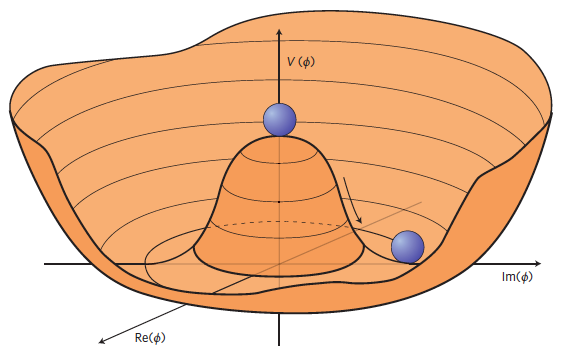
\includegraphics[width=0.45\textwidth]{figures/Intro/higgspotential.png}
    \caption{Higgs potential~\cite{Ellis2015}}
    \label{fig:higgsPotential}
\end{figure}
Therefore, the neutral component ($\phi_3$) of the doublet field $\Phi$ develops a nonzero vacuum expectation value
\begin{equation}
    {\Braket\Phi}_0 = \Braket{0|\Phi|0}=\frac{1}{\sqrt{2}}
        \begin{bmatrix}
        0   \\
        v   \\
        \end{bmatrix}
        with~
        v=-
        \begin{bmatrix}
        \frac{\mu^2}{\lambda}
        \end{bmatrix}
        ^{1/2}
\end{equation}
Now by using the unitarity gauge\footnote{It removes the unphysical degree of freedom} means of proper gauge transformation of the field we get
\begin{equation}
    \Phi (x)=\frac{1}{\sqrt{2}}
        \begin{bmatrix}
        0   \\
        v+h(x)  \\
        \end{bmatrix}
\end{equation}
With $\Phi(x)$ we can expand kinetic term $D_\mu \Phi)^{\dagger} (D_\mu \Phi)=|D_\mu \Phi|^2$ of lagrangian
\begin{eqnarray}\label{mat3}
    |D_{\mu} \Phi|^2 & = & |(\partial_{\mu}-ig_2\frac{\tau_a}{2}W^a_{\mu}-ig_1 \frac{Y_H}{2}B_{\mu})\Phi|^2 \nonumber \\
            & = & \frac{1}{2}(\partial_\mu H)^2+\frac{1}{8}g^2_2(v+H)^2|W^1_{\mu}+iW^2_\mu|^2+\frac{1}{8}|g_2W^3_\mu-g_1B_\mu|^2
\end{eqnarray}
Lets define the new fields $W^{\pm}_\mu$ and $Z_\mu$ [$A_\mu$ is the field orthogonal to $Z_\mu$]:
\begin{equation}
    W^{\pm}=\frac{1}{\sqrt{2}}(W^1_\mu \mp iW^2_\mu),~Z_\mu=\frac{g_2W^3_\mu-g_1B_\mu}{\sqrt{g^2_2+g^2_1}},~A_\mu=\frac{g_2W^3_\mu+g_1B_\mu}{\sqrt{g^2_2+g^2_1}}
\end{equation}
Now pic the term from equation~\ref{mat3} which are bilinear in the fields $W^\pm,Z,A$:
\begin{equation}
    M^2_wW^+_\mu W^{-\mu},~\frac{1}{2}M^2_z Z_\mu Z^\mu,~and~\frac{1}{2}M^2_AA_\mu A^\mu
\end{equation}
Then we noted that W and Z boson have acquired masses, while the photon is still massless
\begin{equation}
    M_w=\frac{1}{2}vg_2,~M_z=\frac{1}{2}v\sqrt{g^2_2+g^2_1},~M_A=0
\end{equation}
So, by spontaneously breaking the symmetry, three Goldstone bosons have been absorbed by the $W^{\pm}$ and Z boson to form their longitudinal components and to get their masses. Since the U(1) symmetry is still unbroken, the photon which is its generator, remains massless.

Now we established that the Higgs mechanism generates the mass for the vector boson. So, now it following the nature.
% But for the Higgs mechanism to be validated Higgs boson should be found experimentally. In July 2012, we found a Higgs like boson. But, is it the Higgs of SM or something else we can say now because of the uncertainty and statistical error involved in the present analysis. 

% So, What are the possible ways to investigate it?

% Basically there are two possible ways to investigate it. First, we should try to study the coupling of the Higgs boson with different particle (top quark is the best candidate). Secondly, we should try to study the vector boson scattering.

% subsection brief_introduction_to_higgs_mechanism (end)

% section brief_introduction_of_sm (end)

\section{Vector Boson Scattering} % (fold)
\label{sec:vector_boson_scattering}
% To understand the structure of electroweak symmetry breaking, one of most important process is the study of vector boson scattering at the LHC. This includes both triple and quartic gauge couplings and the Higgs channels. In the VBS process the initial quarks emits the gauge bosons which interacts with each other and decay afterwards. This is shown in Fig.~\ref{}.
As discussed in the previous section, the VBS is one of important measurements to perfom at LHC. As we know that the VBS includes both triple and quartic gauge coupling. In VBS, the radiated gauge bosons by quark from the two protons and interact with each other and decay afterwards. The feynman diagram corresponding to the VBS is shown in fig.~\ref{fig:VBF_vv_vv}.
\begin{figure}[!htbp]
    \centering
    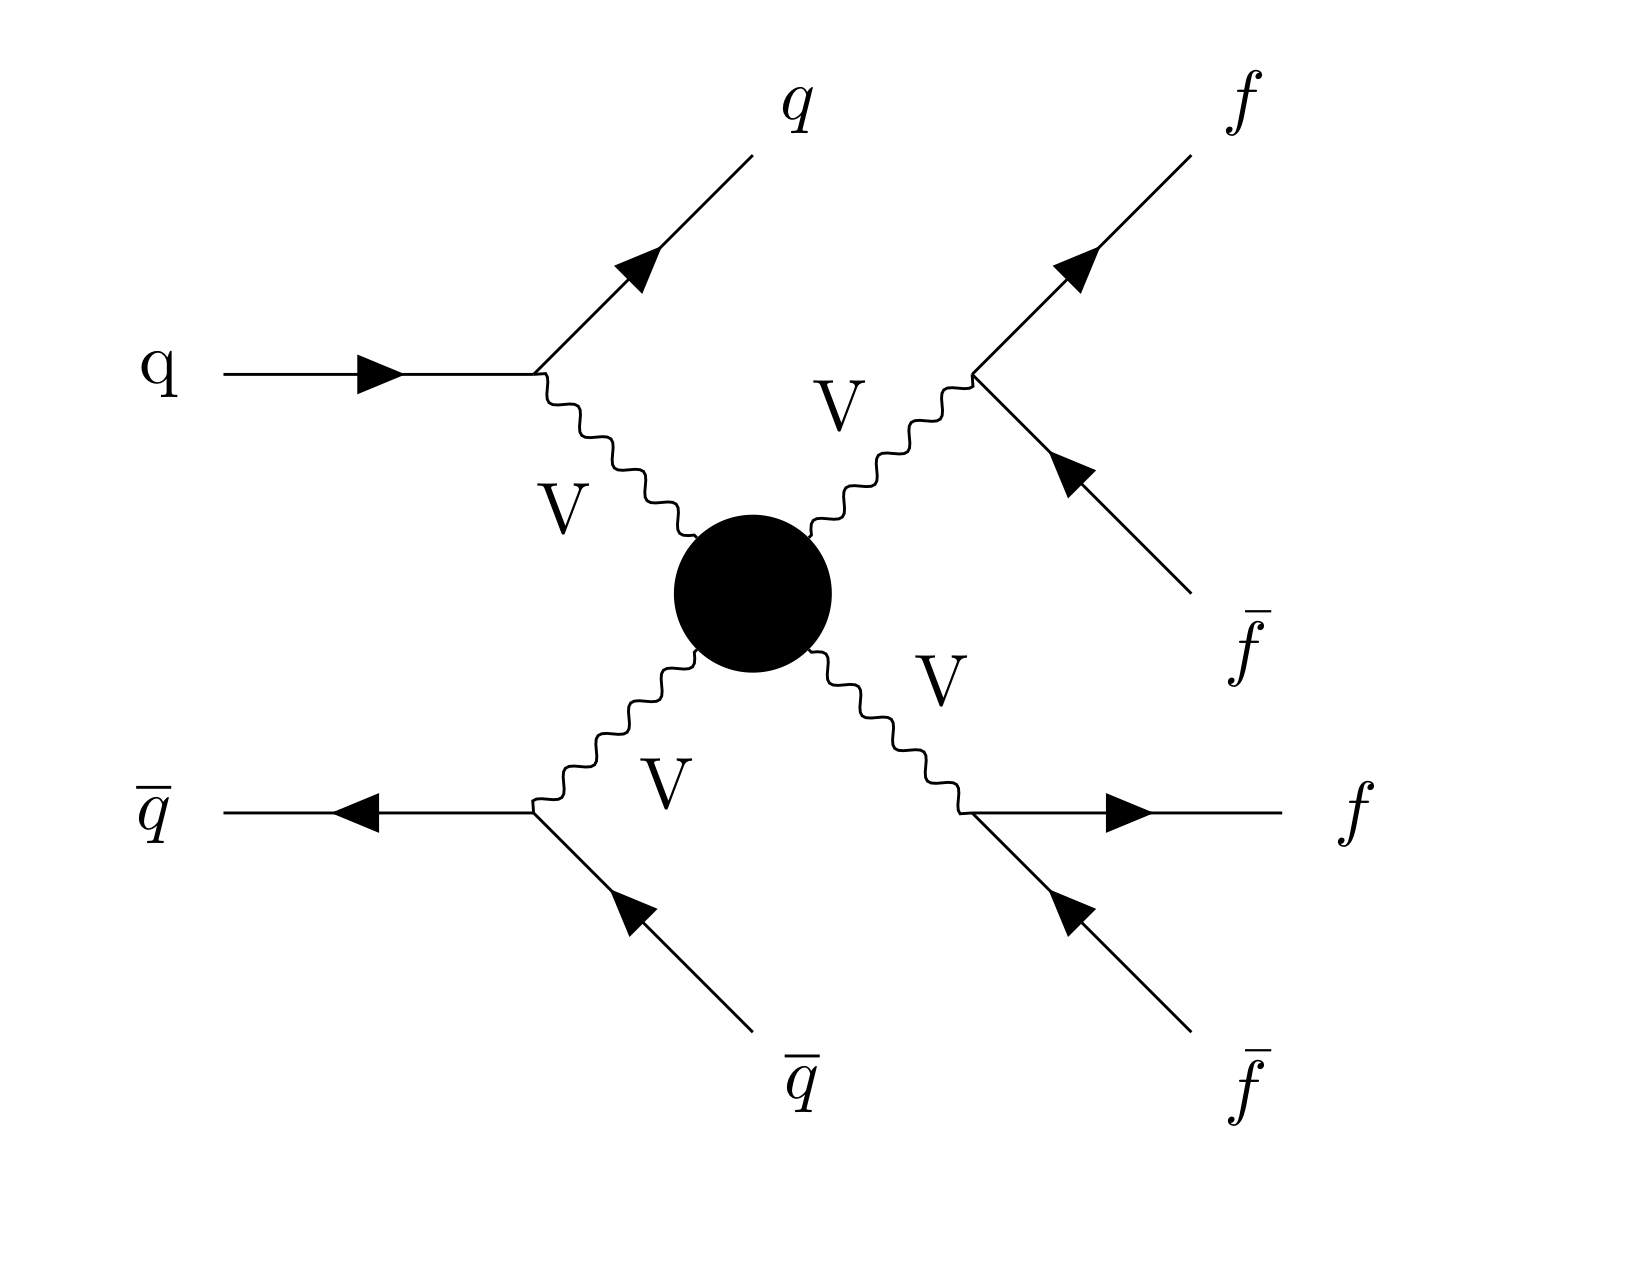
\includegraphics[width=0.45\textwidth]{Pictures/VBF_VV_VV.png}
    \caption{VBS diagram}
    \label{fig:VBF_vv_vv}
\end{figure}

There are several different ways by which the gauge bosons can interact via a quartic vertices or exchange of $Z$ or $\gamma$ or $W$ or a Higgs boson. This is shown using the feynman diagram in Fig.~\ref{fig:VBF_vv_all}
\begin{figure}[!htbp]
    \centering
    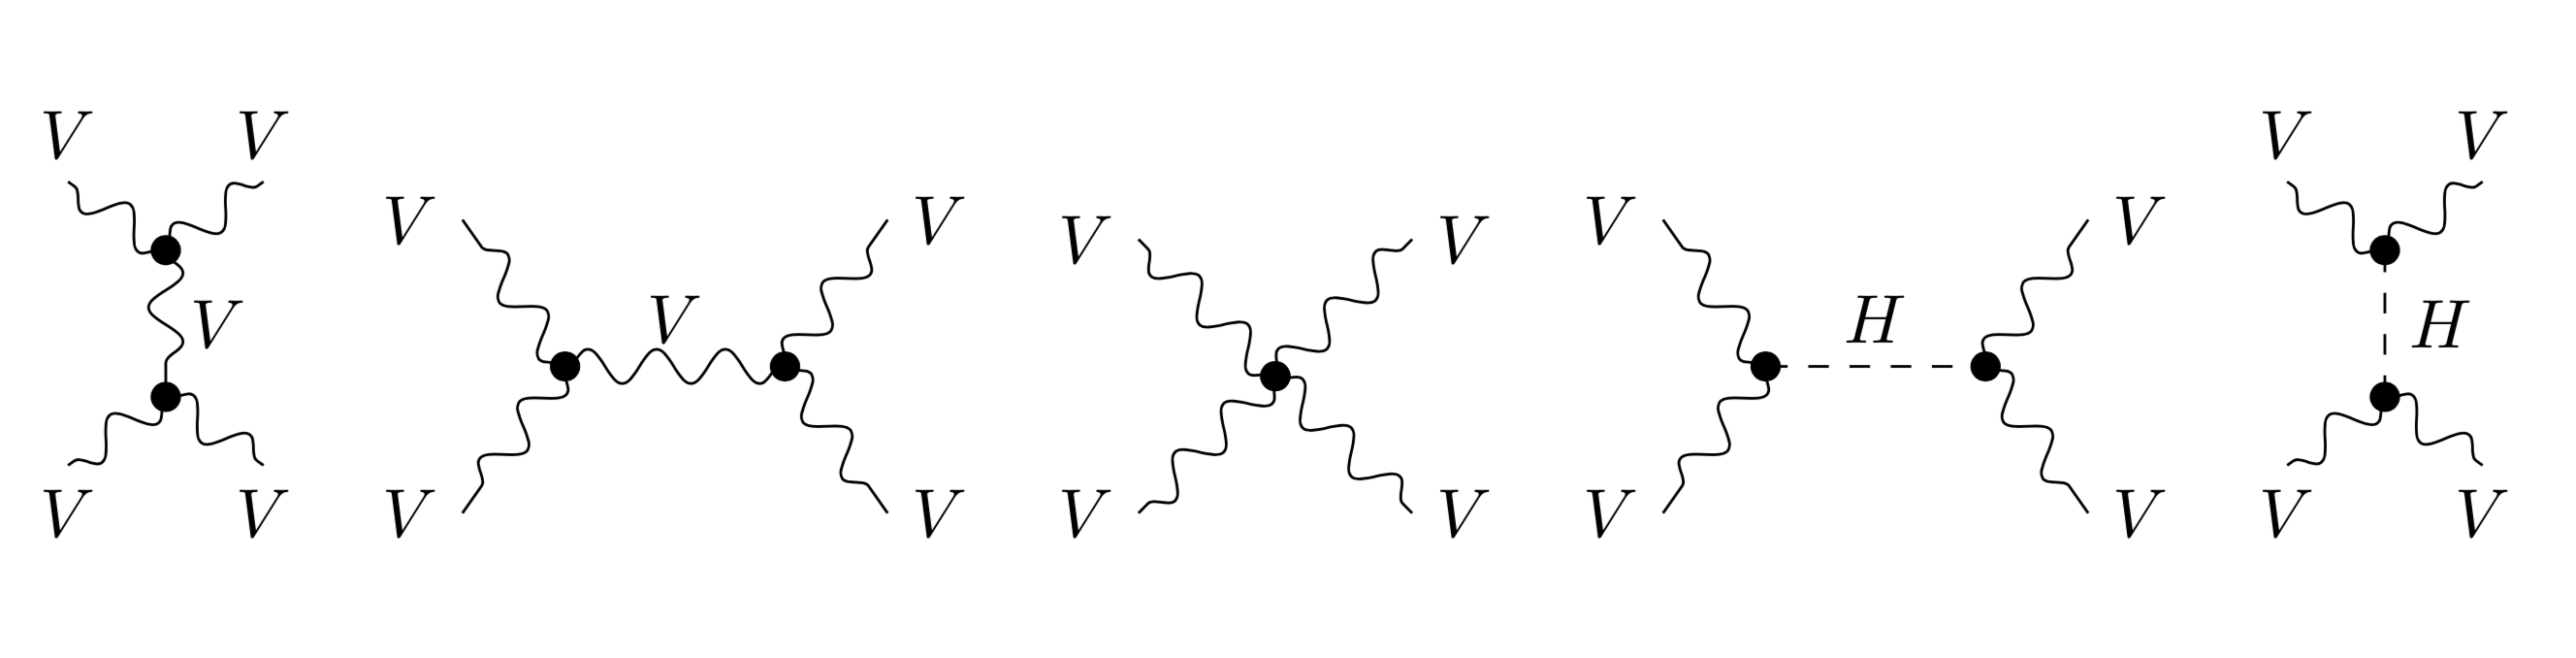
\includegraphics[width=0.95\textwidth]{Pictures/VBF_all.png}
    \caption{VBS diagram}
    \label{fig:VBF_vv_all}
\end{figure}

Vector Boson Scattering requires six weak vertices, so it is a $\mathcal{O}(\alpha^6_W)$ process with a small cross section compared to most of the processes observed at the LHC. One one another difficulties is that we could not generate only $\mathcal{O}(\alpha^6_W)$ process for VBS alone from any available generator in a gauge invariant way. Along with the VBS diagrams it contains lots of other feynman diagrams, as shown in Fig.~\ref{archana}.
\begin{figure}[htbp]
    \centering
    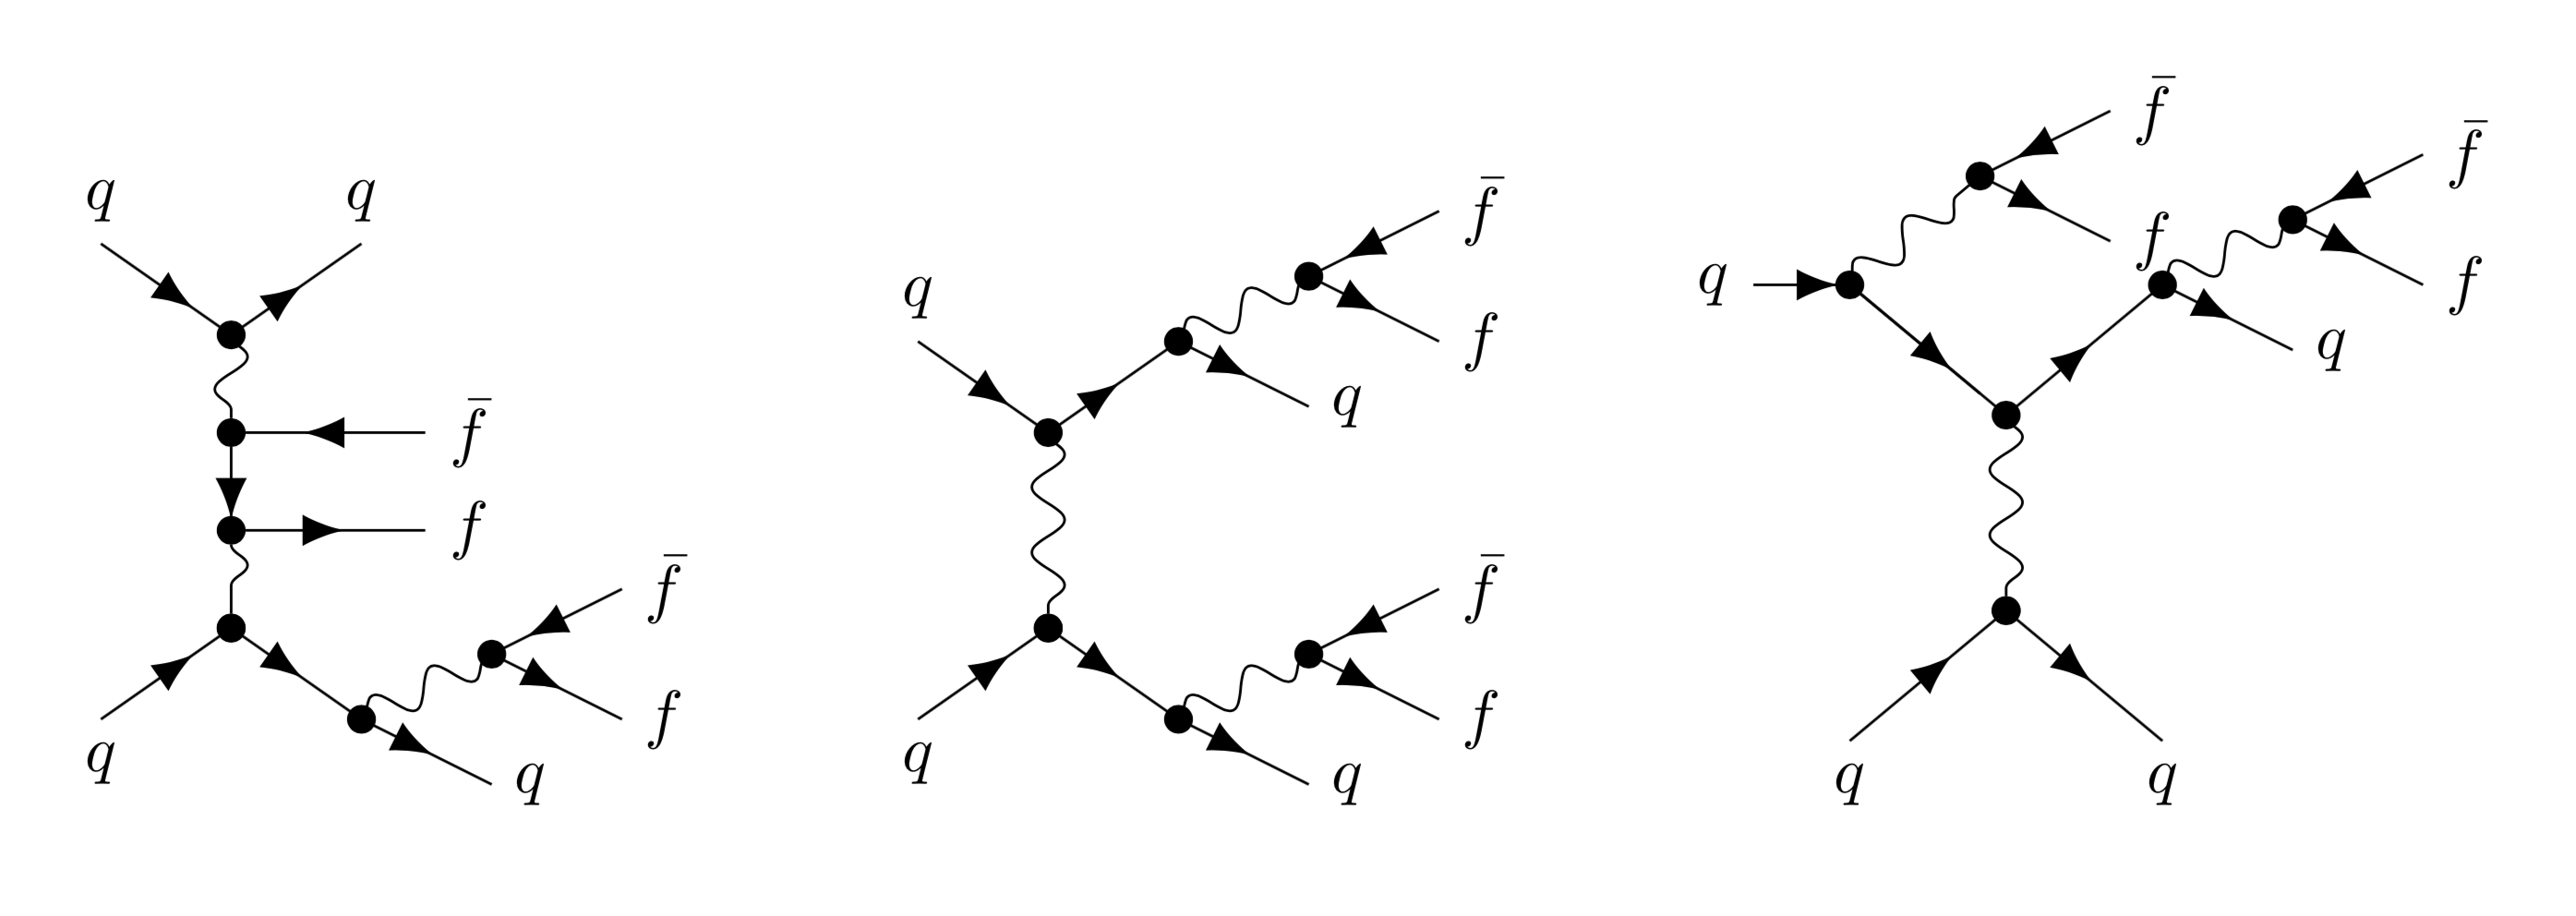
\includegraphics[width=0.95\textwidth]{Pictures/non-vbs.png}
    \caption{caption}
    \label{archana}
\end{figure}
\begin{figure}[htbp]
    \centering
    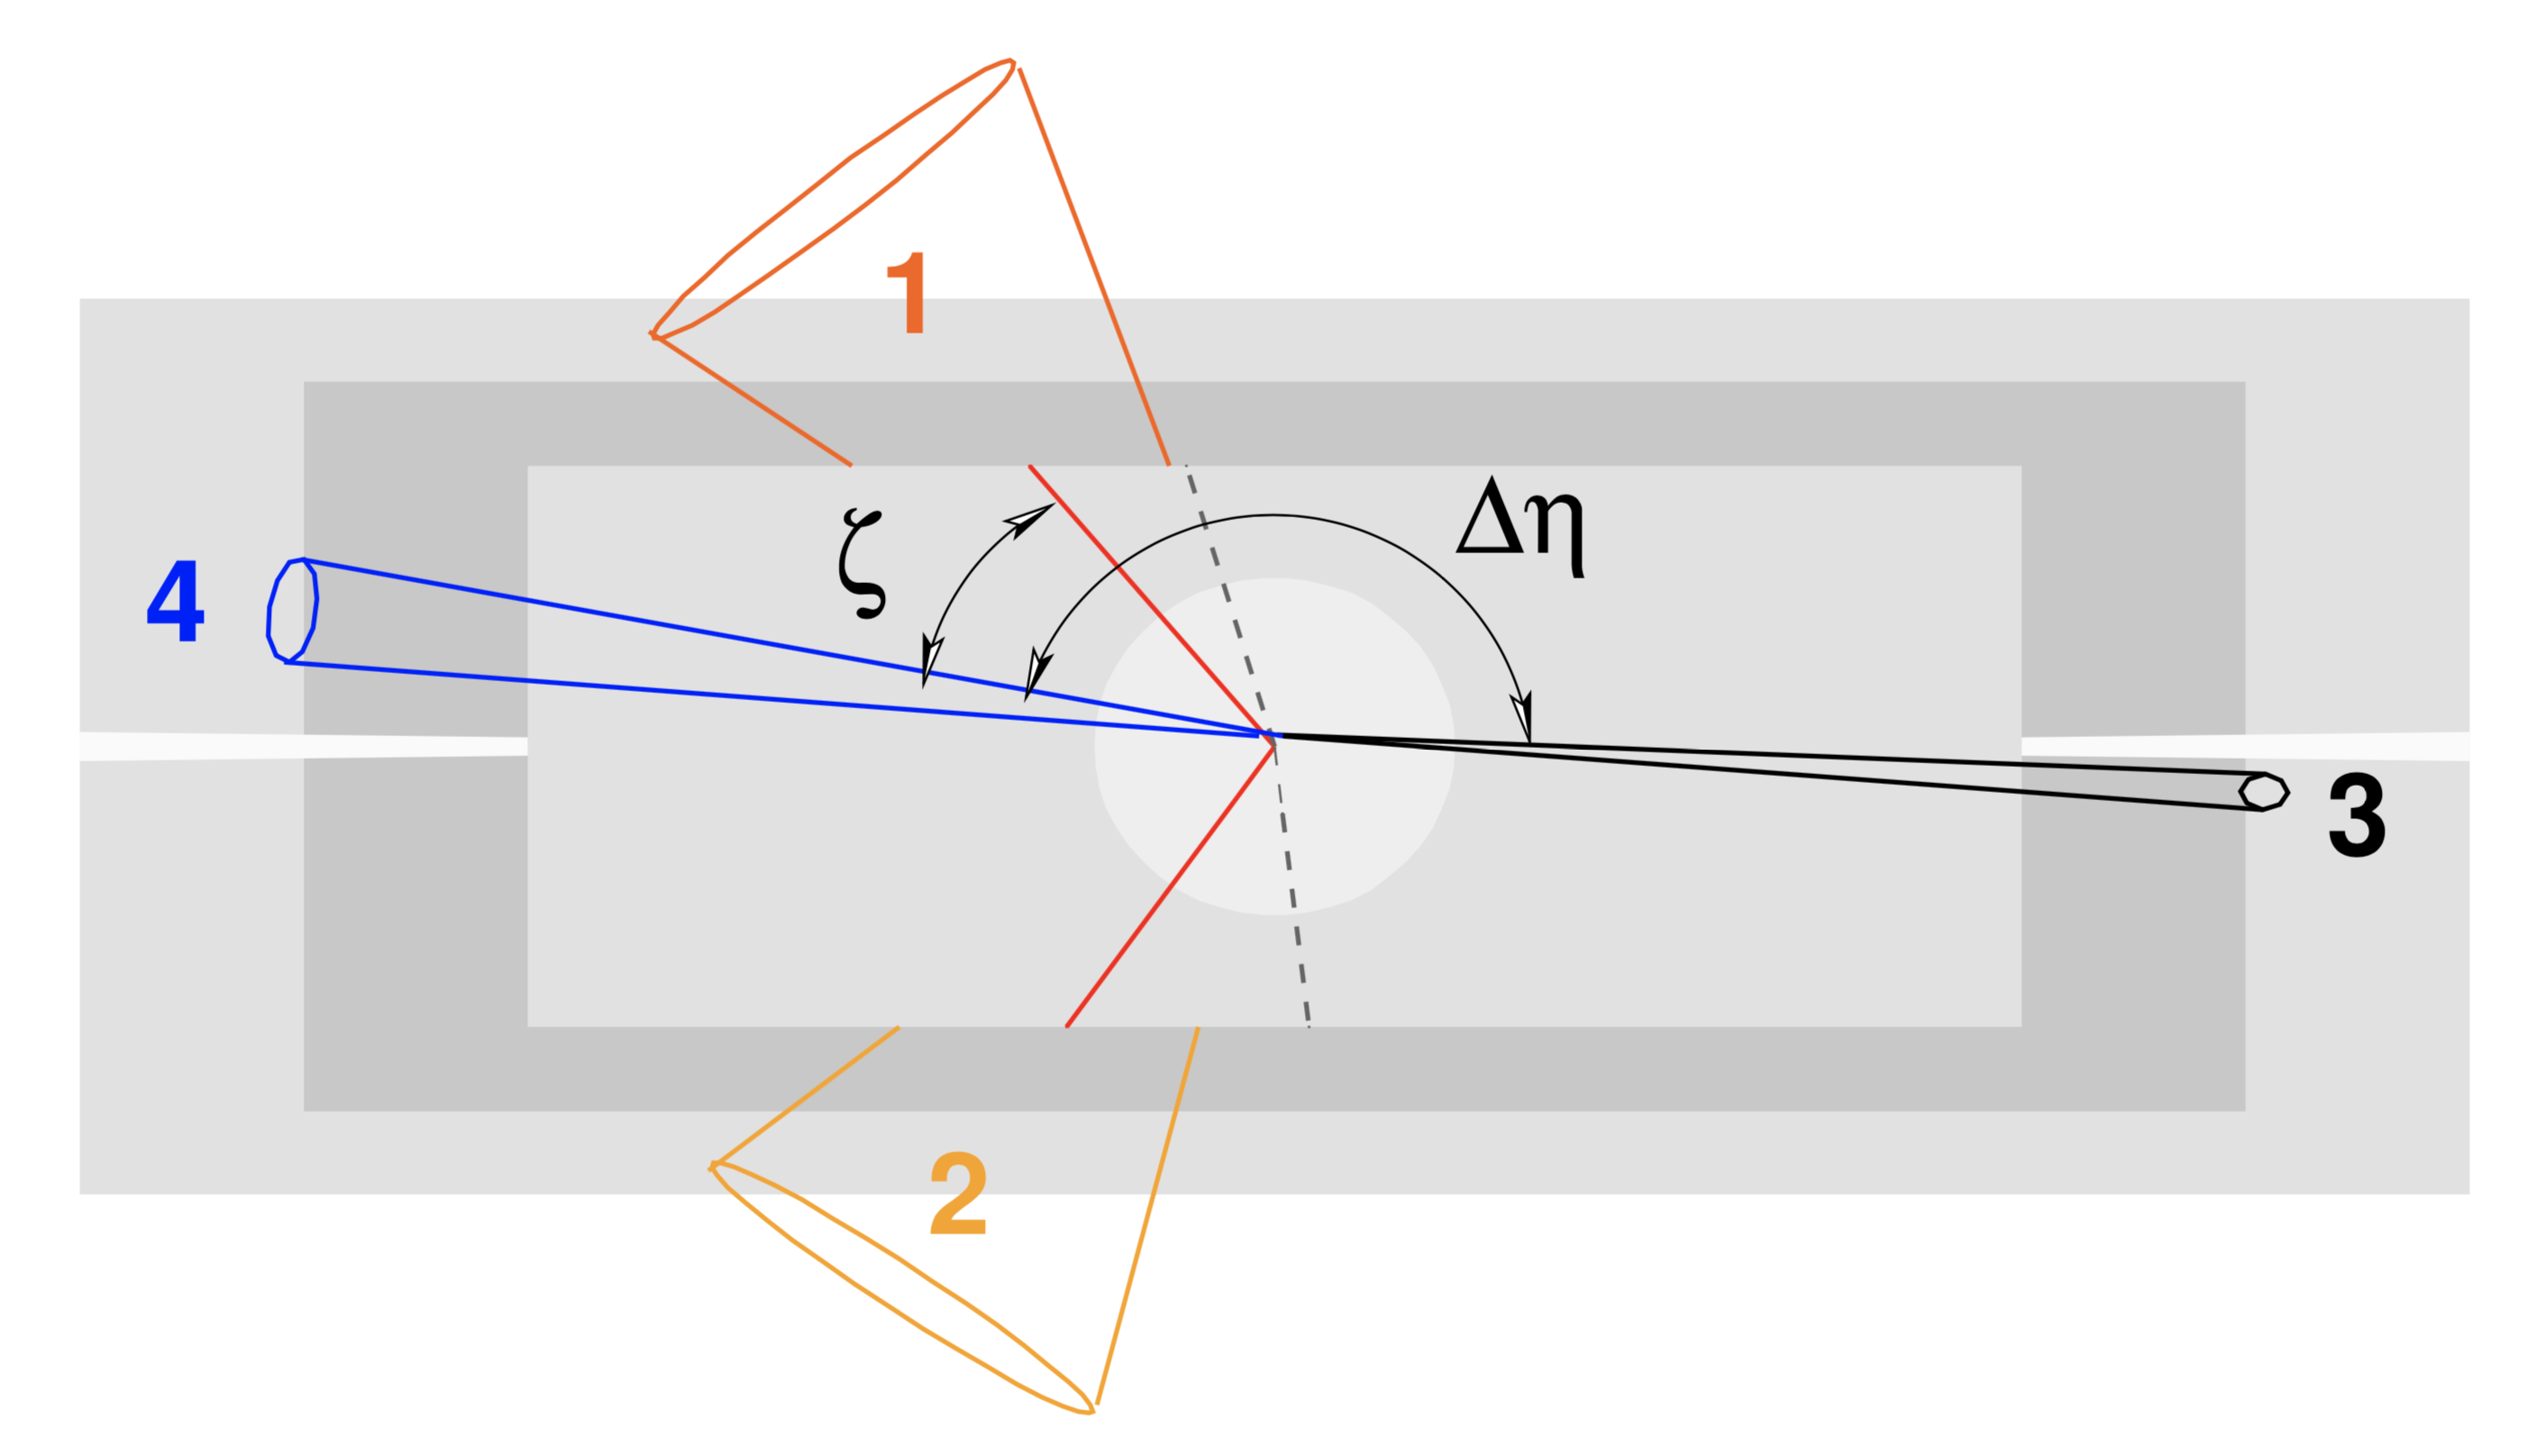
\includegraphics[width=0.95\textwidth]{Pictures/vbs_detector.png}
    \caption{caption}
    \label{fig:vbs_detector}
\end{figure}


The one of important signature of VBS are the two jets in the forward pseudo-rapidity region, called as tagging jets, resulting from the quark emitting the gauge bosons. Thus, the pseudo-rapidity between the tagging jets is expected to be large.

Furthermore, there are different modes of decay of w-bosons like $WW \rightarrow l \nu l\nu $, $WW \rightarrow jj jj $, and $WW \rightarrow l \nu jj$. The leptonic channel is considered to have less background specially if working with same sign W-bosons but it has very less cross-section than semi-leptonic or fully hadronic. While the fully hadronic channel has comparatively larger cross-section but it suffers from huge QCD background. Thus, one of best way to work with semi-leptonic channel which has larger branching fraction than fully leptonic and comparatively lesser background than fully-hadronic, for which the analysis was performed and the details are given in Section~\ref{cha:physics_analysis}.

% Due to experimental limitations it was not yet observed.
% 

% section vector_boson_scattering (end)

\section{anomalous Quartic Gauge Coupling} % (fold)
\label{sec:anomalous_quartic_gauge_coupling}
Up to now the SM is in good agreement with experiment but it is possible that the SM is correct up to an unknown centre of mass energy scale $\Lambda$.
Thus, it is possible that the new effects or completely new physics lies above this scale but it could be seen as an indirect effects on the currently accessible energy.
One of possible way is to build an Effective Field Theory (EFT) to parametrize the effects of high energy scale effect on the energy scale available to us. This introduces new degree of freedom to the SM.

The new effective lagrangian using the EFT is
% \begin{equation}
%     \Lagr_{eff} = \Lagr_{SM} + \sum_{d>4} \sum_i{\frac{c_i^{(d)}}{\Lambda^{d-4}}\mathcal{O}_i^{d}},
% \end{equation}

\begin{equation}
    \Lagr_{eff} = \Lagr_{SM} + \sum_{i=www,w,B, \phi W, \phi B} \frac{c_i}{\Lambda^2} {\Oo}_i + \sum_{j=0,1}\frac{f_{S,j}}{\Lambda^4} \Oo_{S,j} + \sum_{j=0,...,9}\frac{f_{T,j}}{\Lambda^4} \Oo_{T,j}  + \sum_{j=0,...,7}\frac{f_{M,j}}{\Lambda^4} \Oo_{M,j} ,
\end{equation}
here, $\Lambda$ is the new physics scale, the parameter $c_i$, is the dimensionless coupling-strength coefficient of order $\Oo(1)$ and $f_{s,j}$, $f_{T,j}$ and $f_{M,j}$ are for the dimensionless coupling-strength coefficient for the quartic gauge couplings. Also, in EFT at $\Lambda \rightarrow \inf$ the effective Lagrangian should reduce to the SM one.

Due to the higher dimension these operators $\mathcal{O}$ have coefficients of inverse power of mass so the operators with the lowest dimension are dominant. Most of the SM operators are of dimension four and since only operators with even dimension satisfy conservation of lepton and baryon number the new operators have to be at least dimension six operators~\cite{Degrande2013a}. 
These new operators effect also double and triple gauge boson couplings; these can be studied more easily in other processes. \todo[inline]{Rewrite this para...}.

Dimension eight operators have no effects in double or triple couplings so they have to be searched for in quartic gauge couplings. Vector Boson Scattering allows these examinations. In general the following are the possible operators for the quartic gauge boson vertex:

\subsubsection{Operators containing only $D_\mu \phi$} % (fold)
\label{ssub:operators_containing_only_}
In this category there are two independent operators. They are:
\begin{eqnarray}
    \mathcal{O}_{S,0}=\Big[(D_{\mu}\phi)^{\dagger}\times D_{\nu}\phi) \Big]\times \Big[(D^{\mu}\phi)^{\dagger}D^{\nu}\phi \Big], \\
    \mathcal{O}_{S,1}=\Big[(D_{\mu}\phi)^{\dagger}\times D^{\mu}\phi)\Big]\times \Big[(D_{\nu}\phi)^{\dagger} D^{\nu}\phi\Big],
\end{eqnarray}
where the Higgs covarient derivative is given as
\begin{equation}\label{eq:covarient_derivative_qgc}
     D_\mu = \partial_\mu + i\frac{g'}{2}B_\mu + ig_w W^i_{\mu} \frac{T^i}{2}
 \end{equation} 
 and the field strength tensors of the $SU(2)_L$ $(W^i_\mu)$ and $U(1)_Y$  $(B_\mu)$ gauge fields are given as
\begin{eqnarray}\label{eq:fieldstrength_qgc}
    W_{\mu \nu} = \frac{i}{2}g T^i (\partial_\mu W^i_\nu - \partial_\nu W^i_\mu + g \epsilon_{ijk} W^j_\mu W^k_\nu) \\
    B_{\mu \nu} = \frac{i}{2} g' (\partial B_\nu - \partial_\nu B_\mu)
\end{eqnarray}
The operators $\Oo_{S,0}$ and $\Oo_{S,1}$ contains the quartic gauge coupling for process $\ww \ww$, $\ww \zz$ and $\zz \zz$ interactions which do not depend on the gauge boson momenta. 
% subsubsection operators_containing_only_ (end)

\subsubsection{Operators containing $D_{\mu}\phi$ and two field strength tensors} % (fold)
\label{ssub:operators_containing_}
The quartic gauge coupling is also generated by using the two electroweak field strength tensors and two covariant derivatives of the Higgs doublet as:
\begin{eqnarray}
\mathcal{O}_{M,0}=Tr\Big[W_{\mu\nu}W^{\mu\nu}]\times \Big[(D_{\beta}\phi)^{\dagger}D^{\beta}\phi] \\
\mathcal{O}_{M,1}=Tr\Big[W_{\mu\nu}W^{\nu\beta}]\times \Big[(D_{\beta}\phi)^{\dagger}D^{\mu}\phi]\\
\mathcal{O}_{M,2}=\Big[B_{\mu\nu}B^{\mu\nu}]\times \Big[(D_{\beta}\phi)^{\dagger}D^{\beta}\phi]\\
\mathcal{O}_{M,3}=\Big[B_{\mu\nu}B^{\nu\beta}]\times \Big[(D_{\beta}\phi)^{\dagger}D^{\mu}\phi]\\
\mathcal{O}_{M,4}=\Big[(D_{\mu}\phi)^{\dagger}W_{\beta\nu}D^{\mu}\phi]\times B^{\beta\nu}\\
\mathcal{O}_{M,5}=\Big[(D_{\mu}\phi)^{\dagger}W_{\beta\nu}D^{\nu}\phi]\times B^{\beta\mu}\\
\mathcal{O}_{M,6}=\Big[(D_{\mu}\phi)^{\dagger}W_{\beta\nu}W^{\beta\nu}D^{\mu}\phi]\\
\mathcal{O}_{M,7}=\Big[(D_{\mu}\phi)^{\dagger}W_{\beta\nu}W^{\beta\nu}D^{\mu}\phi]
\end{eqnarray}
Here, the field strength tensors $W_{\mu \nu}$ and $B_{\mu \nu}$ is defined as Eq.~\ref{eq:fieldstrength_qgc}. This class of operators of the quartic gauge-boson interaction depends on the vector boson momenta due to the presence of the field strength tensors.
% subsubsection operators_containing_ (end)

\subsubsection{Operators containing only field strength tensors} % (fold)
\label{ssub:operators_containing_only_field_strength_tensors}
In this class only the field strength tensors lead to the anomalous quartic couplings, which is given by following operators:
\begin{eqnarray}
    \mathcal{O}_{T,0}=Tr\Big[W_{\mu\nu}W^{\mu\nu}]\times Tr\Big[W_{\alpha\beta}W^{\alpha\beta}]\\
    \mathcal{O}_{T,1}=Tr\Big[W_{\alpha\nu}W^{\mu\beta}]\times Tr\Big[W_{\mu\beta}W^{\alpha\nu}]\\
    \mathcal{O}_{T,2}=Tr\Big[W_{\alpha\mu}W^{\mu\beta}]\times Tr\Big[W_{\beta\nu}W^{\nu\alpha}]\\
    \mathcal{O}_{T,5}=Tr\Big[W_{\mu\nu}W^{\mu\nu}]\times B_{\alpha\beta}B^{\alpha\beta}\\
    \mathcal{O}_{T,6}=Tr\Big[W_{\alpha\nu}W^{\mu\beta}]\times B_{\mu\beta}B^{\alpha\nu}\\
    \mathcal{O}_{T,7}=Tr\Big[W_{\alpha\mu}W^{\mu\beta}]\times B_{\beta\nu}B^{\nu\alpha}\\
    \mathcal{O}_{T,8}=B_{\nu\mu}B^{\nu\mu}B_{\alpha\beta}B^{\alpha\beta}\\
    \mathcal{O}_{T,9}=B_{\alpha\mu}B^{\mu\beta}B_{\beta\nu}B^{\nu\alpha}
\end{eqnarray}
The last two operators $\mathcal{O}_{T,8}$ and $\mathcal{O}_{T,9}$ are the operators which contains only the neutral electroweak gauge bosons.
The list of all quartic vertices modified by all the dimension-8 operators are listed in Table~\ref{table:aQGC_alloperator}.

\begin{table}
% \vspace{-5.2em}
\centering
% \begin{tabular}[!htbp]{|p{2.5cm} | p{1.5cm} |p{1.3cm} |p{1cm} |p{1.3cm} |p{1.4cm} |p{1cm} |p{1cm}| p{1cm} |p{1cm}|}
\begin{tabular}[!htbp]{|p{1.8cm} | c  |c  |c  |c  |c  |c  |c | c  |c |}
\hline
    & WWWW & WWZZ & ZZZZ & WWAZ & WWAA & ZZZA & ZZAA & ZAAA & AAAA \\
\hline
$f_{S,0}$, $f_{S,1}$ &$\times$ & $\times$&$\times$ & & & & & & \\
\hline
$f_{M,0}$, $f_{M,1}$, $f_{M,6}$, $f_{M,7}$  &$\times$ &$\times$ &$\times$ &$\times$ &$\times$ &$\times$ &$\times$ & & \\
\hline
$f_{M,2}$, $f_{M,3}$, $f_{M,4}$, $f_{M,5}$  & &$\times$ &$\times$ &$\times$ &$\times$ &$\times$ &$\times$ & & \\
\hline
$f_{T,0}$, $f_{T,1}$, $f_{T,2}$ &$\times$ &$\times$ &$\times$ &$\times$ &$\times$ &$\times$ &$\times$ &$\times$ &$\times$ \\
\hline
$f_{T,5}$, $f_{T,6}$, $f_{T,7}$ & &$\times$ &$\times$ &$\times$ &$\times$ &$\times$ &$\times$ &$\times$ &$\times$ \\
\hline
$f_{T,8}$, $f_{T,9}$  & & &$\times$ & & &$\times$ &$\times$ &$\times$ &$\times$ \\
\hline
\end{tabular}
\caption{Quartic vertices modified by the different operators are marked with $\times$.}
\label{table:aQGC_alloperator}
\end{table}

% subsubsection operators_containing_only_field_strength_tensors (end)

% section anomalous_quartic_gauge_coupling (end)

\section{George-Machak Model} % (fold)
\label{sec:george_machak_model}
As discussed in the previous sections it is important to undurstand the structure for the $SU(2) \times U(1)$ breaking physics and its experimental signatures. For this the one of important study is to measure the quartic gauge boson couplings along with that how the gauge bosons couples with the Higgs bosons. If the Higgs boson mass is large enough it can easily decays predominantly into the two gauge bosons.

In this section we will discuss one of such model where the doubly charged Higgs particles appear and measure the extent to which the gauge bosons can couples.

The Higgs doublet of the SM is given as:
\begin{equation}
      \Phi=
        \begin{bmatrix}
        \phi^+  \\
        \phi^0  \\
        \end{bmatrix}
\end{equation}

and the new triplet Higgs field is given as

\begin{equation}
    \chi = 
        \begin{bmatrix}
        \chi^0     & \zeta^+    &   \chi^{++} \\
        \chi^-     & \zeta^0    &   \chi^{+} \\
        \chi^{--}  &  \zeta^-   &   \chi^{0*} \\
        \end{bmatrix}
\end{equation}

This triplet field satisfies the equation

\begin{equation}
    \chi^{\dagger} = C~ \chi ~C
\end{equation}

where,
\begin{equation}
    C = 
    \begin{bmatrix}
        0   &   0   & 1 \\
        0   &   -1  & 0 \\
        1   &   0   & 0 \\
    \end{bmatrix}
\end{equation}

The kinetic energy term for the higgs triplet field along with the doublet field for $SU(2) \times SU(1)$ is
\begin{equation}
    (D^\mu \phi)^{\dagger} D_{\mu} \phi + \frac{1}{2}tr\Big[ (D^{\mu} \chi)^{\dagger} D_{\mu} \chi \Big],
\end{equation}
where
\begin{eqnarray}
    D^\mu \phi & = & \partial^{\mu}\phi + ig W^{\mu}_{a} \tau_{a} \frac{1}{2} \phi + i g' \chi^{\mu} \frac{1}{2} \phi, \nonumber \\
    D^\mu \chi & = & \partial^{\mu}\chi + ig W^{\mu}_{a} t_{a} \frac{1}{2} \chi - i g' X^{\mu} ~\chi ~t_3, \nonumber \\
    g & = & e/sin\theta,~~~~~ g' = e/cos \theta, \\ 
\end{eqnarray}

where,
\begin{equation}
    t_1 = \sqrt{\Big(\frac{1}{2}\Big)}
        \begin{bmatrix}
        0   &   1   &   0 \\
        1   &   0   &   1 \\
        0   &   1   &   0 \\
        \end{bmatrix},~~~
    t_2 = \sqrt{\Big(\frac{1}{2}\Big)}
        \begin{bmatrix}
        0   &   -i   &   0 \\
        i   &   0   &   i \\
        0   &   i   &   0 \\
        \end{bmatrix},~~~
    t_3 = 
        \begin{bmatrix}
        1   &   0   &   0 \\
        0   &   0   &   0 \\
        0   &   0   &   1 \\
        \end{bmatrix},
\end{equation}
% section george_machak_model (end)

\section{Georgi-Machacek Model} % (fold)
\label{sec:georgi_machacek_model}
In Georgi-Machacek (GM) model along with the SM Higgs doublet $\Phi = (\phi^+,~\phi^0)^T$ having hypercharge\footnote{$Q = T^3 + \frac{Y}{2}$}, Y = 1, alongwith a real triplet $(\zeta^+,~\zeta^0,~-\zeta^+*)^T$ with Y = 0 and a complex triplet $(\chi^{++},~\chi^+,~\chi^0)^T$ with Y = 2 is introduced.

Also, a constraint from the electroweak parameter, $\rho$, also known as ``\textit{Custodial Symmetry}'', is imposted by the global $SU(2)_L \times SU(2)_R$ symmetry upon the scalar potential. The parameter $\rho$ is given as
\begin{equation}
    \rho = \frac{M_W}{M_Z ~ cos(\theta)} = 1,
\end{equation}
where, $\theta$ is the weak mixing angle.
A isospin doublet of the $SU(2)_L \times SU(2)_R$ is given as
\begin{equation}
    \Phi = 
    \begin{bmatrix}
        \phi^{0*} &  \phi^+ \\
        -\phi^{+*} & \phi^0 \\
    \end{bmatrix}
\end{equation}
and the triplet  Higgs field is given as
\begin{equation}
    X = (\epsilon_3 \chi*,~\zeta,~\chi) = 
    \begin{bmatrix}
        (\chi^0)^*     &   \zeta^+     &   \chi^{++} \\
        -(\chi^{+})^*    &   \zeta^0     &   \chi^+    \\
        (\chi^{++})^*  &   (-\zeta^+)^*   &   \chi^0    \\
    \end{bmatrix}
\end{equation}
The vacum expectation values (vev) for the $\Phi$
\begin{equation}
    \Braket{\Phi} = \frac{V_\phi}{\sqrt{2}} \mathbb{1}_{2\times 2}
\end{equation}
and for the field $X$ is 
\begin{equation}
    \Braket{X}  = v_x \mathbb{1}_{3\times 3}
\end{equation}
where, $\mathbb{1}$ is the unit matrix and the W and Z boson to be massless provides a condition that

\begin{equation}
    v_\phi^2 + 8v_{\chi}^2 = v = \frac{1}{\sqrt{2}G_F} \approx (246~GeV)^2
\end{equation}

The most general gauge invariant potential involving these fields that preserve the custodial symmetry is given as
\begin{eqnarray}
    V{\Phi,X} & = & \frac{\mu_2^2}{2}Tr(\Phi^{\dagger}\Phi) + \frac{\mu_3^2}{2}Tr(X^{\dagger}X)  \nonumber \\
            & & + \lambda_1\Big[ Tr(\phi^\dagger \phi)\Big] + \lambda_2 Tr\Big[ (\phi^{\dagger} \phi) Tr(X^{\dagger}X) \Big] \nonumber \\
            & & + \lambda_3 Tr(X^{\dagger}XX^{\dagger}X) + \lambda_4 \Big[ Tr(X^{\dagger}X) \Big]^2  \nonumber \\
            & & -\lambda_5 Tr(\phi^{\dagger} \tau^a \phi \tau^b) Tr(X^{\dagger} t^a X t^b)   \nonumber \\
            & & -M_1 Tr(\phi^{\dagger} \tau^a \phi \tau^b) (UXU^{\dagger})_{ab} \nonumber \\
            & & -M_2 Tr(X^{\dagger} t^a X t^b)(UXU^{\dagger})_{ab}
\end{eqnarray}
where $\tau^a = \frac{\sigma^a}{2}$,
\begin{equation}
    t^1=\frac{1}{\sqrt{2}}
        \begin{bmatrix}
        0   &   1 & 0 \\
        1   &   0 & 1 \\
        0   &   1 & 0   \\
        \end{bmatrix},~~
    t^2 = \frac{1}{\sqrt{2}}
        \begin{bmatrix}
        0   &   -i & 0 \\
        i   &   0 & -i \\
        0   &   i & 0   \\
        \end{bmatrix},~~
    t^3 = 
        \begin{bmatrix}
        1   &   0 & 0 \\
        0   &   0 & 0 \\
        0   &   0 & -1   \\
        \end{bmatrix},
\end{equation}\

The physical fields generated can be organized by the transformation properties under the custodial SU(2) symmetry into pentaplet and a triplet and two singlets. They are:
\begin{eqnarray}
    \mathbf{Pentaplet}~:&   & H^{++}_5 = \chi^{++} \\
                        &   & H^+_5 = \frac{\chi^+ - \zeta^+}{\sqrt{2}} \\
                        &   & H^0_5 = \sqrt{\frac{2}{3}}\zeta^{0,r} - \sqrt{\frac{1}{3}}\chi^{0,r} \\
                        &   & \\
    \mathbf{Triplet}~:  &   & H^+_3 = -S_H \phi^+ + C_H \frac{\chi^++X^+}{\sqrt{2}} \\
                        &   & H^0_3 = -S_H \phi^{0,i} + C_H \chi^{0,i} \\
                        &   & \\
    \mathbf{Singlet}~:  &   & H^0_1 = \phi^{0,r}\\
                        &   & H^{0'}_1 = \sqrt{\frac{1}{3}}\zeta^{0,r} + \sqrt{\frac{2}{3}} \chi^{0,r},
\end{eqnarray}
where,
\begin{eqnarray}
    S_H = sin(\theta_H) = \frac{2\sqrt{2} v_\chi}{v} \\
    C_H = cos(\theta_H) = \frac{v_\phi}{v}
\end{eqnarray}
Here, within the pentaplets and the triplets, the masses are degenerated at the tree level and are given in terms of the parameters of scalar potential by
\begin{eqnarray}
    m_5^2 & = & \frac{M_1}{4v_\chi} v_{\phi}^2 + 12 M_2 v_{\chi} + \frac{3}{2}\lambda_5 v^2_{\phi} + 8 \lambda_3 v_{\chi}^2 \\
    m_3^2 & = & \frac{M_1}{4v_\chi} v^2 + \frac{\lambda_5}{2} v^2 
\end{eqnarray}
The two custodial singlets will  mix by an angle $\alpha$ to give the two mass egien state $h$ and $H$,
\begin{eqnarray}
    h & = & C_{\alpha} H^0_1 - S_{\alpha} H^{0'}_1 \\
    H & = & S_{\alpha} H^0_1 + C_{\alpha} H^{0'}_1
\end{eqnarray}
where, $C_{\alpha} = cos(\alpha)$ and $S_{\alpha} = sin(\alpha)$. The mixing is controlled by the mass matrix
\begin{equation}
    M^2 = 
        \begin{bmatrix}
            M_{11}^2 & M^2_{12} \\
            M_{12}^2 & M^2_{22} \\
        \end{bmatrix}
\end{equation}
where,
\begin{eqnarray}
    M^2_{11} & = & 8 \lambda_1 v^2_{\phi} \\
    M^2_{12} & = & \frac{\sqrt{2}}{2} v_{\phi} \Big[-M_1 + 4(2\lambda_2 - \lambda_5) v_x \Big] \\
    M^2_{22} & = & \frac{M_1}{4 v_{\chi}}v^2_{\phi} - 6 M_2 v_{\chi} + 8(\lambda_3 + 3\lambda_4) v^2_{\chi}
\end{eqnarray}

Some remarkable feature of the GM model is that the $HWW$ and $HZZ$ coupling may be larger than in the SM. 
The pentaplet Higgs bosons have coupling with the weak bosons while the triplet do not. Thus, the triplet Higgs bosons are said to be gauge-phobic while the pentaplets are known as fermi-phobic.
% The custodial pentaplets have no doublet component and hence they are fermifobic at the tree level.
But these pentaplets can couples to the massive vector boson where the coupling strenght is proportional to the parameter $S_H$.

% section georgi_machacek_model (end)

% \section{Experimental Status} % (fold)
% \label{sec:experimental_status}

% \subsection{aQGC measurements} % (fold)
% \label{sub:aqgc_measurements}

% % subsection aqgc_measurements (end)

% \subsection{GM model} % (fold)
% \label{sub:gm_model}

% subsection gm_model (end)


% section experimental_status (end)



% chapter standard_model_&_vector_boson_scattering (end)